\subsection{User Setting}

User settings in a web application refer to the customizable options and preferences that users can set to personalize their experience within the application.\\

User settings may include options such as language preferences, time zone settings, font size, color schemes, notification preferences, privacy and security settings, and more.\\

These settings can enhance the user experience by allowing users to tailor the application to their specific needs and preferences.\\

User settings are typically accessed via a user profile or settings page within the web application and can be modified at any time by the user.\\

User settings can also include features like account management, password and email settings, and social media integrations.\\

By providing users with control over their experience, web applications can improve user engagement and satisfaction.\\
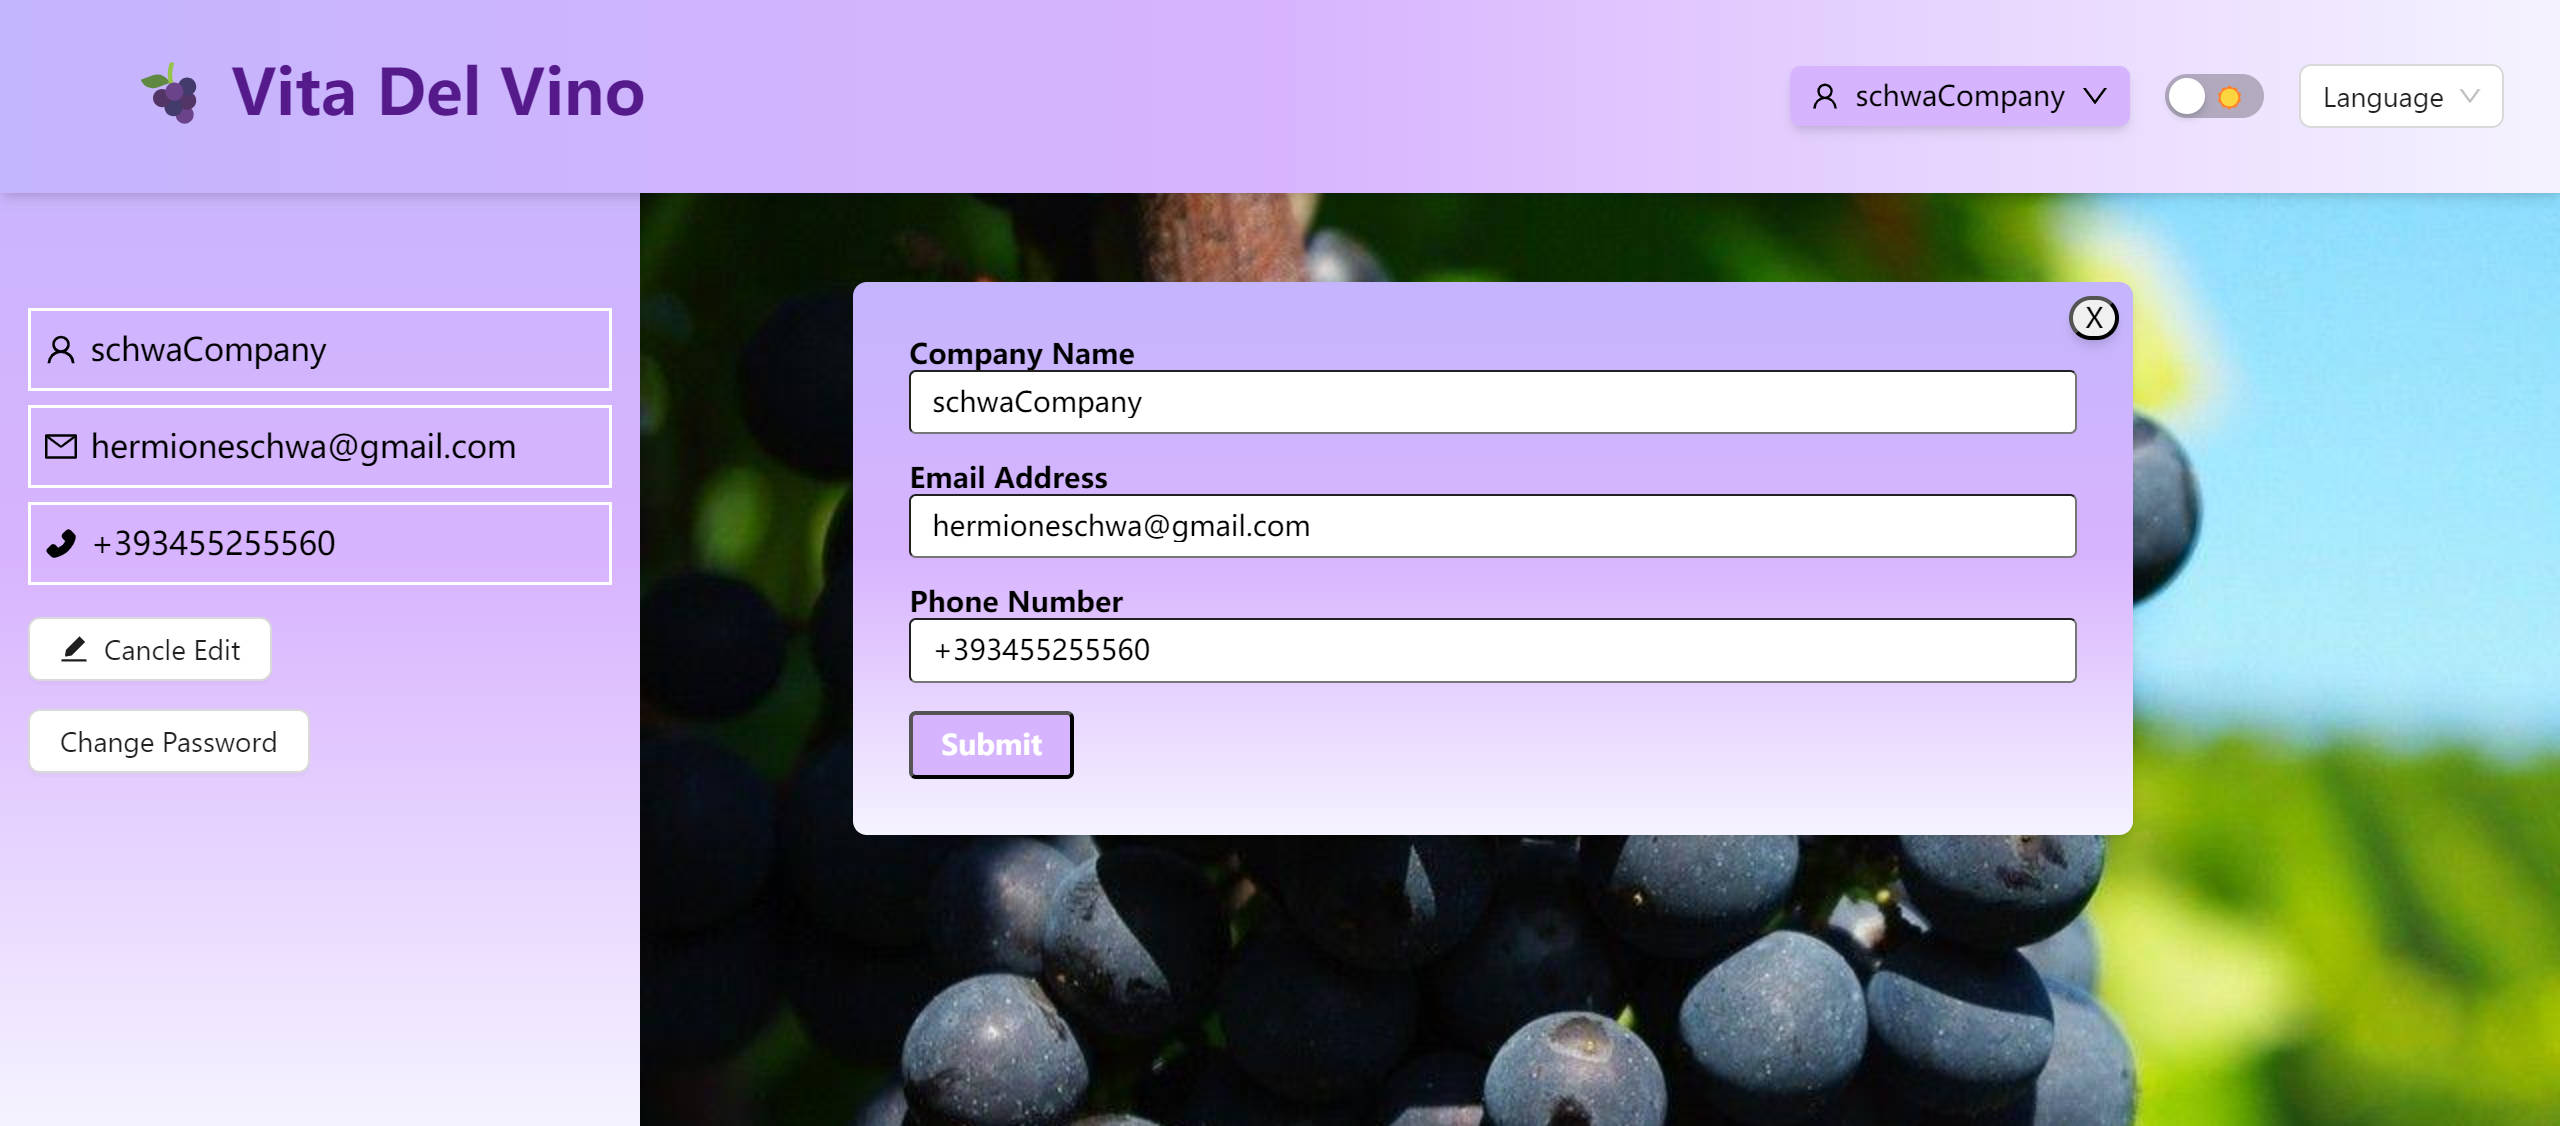
\includegraphics[width=\columnwidth]{images/UserSetting.jpg}

